\chapter{Grundlagen}
\label{cha:Grundlagen}
\section{Grundprinzip und Wärmetransport}
\label{sec:WaermeuebergaengeamSprinklerkopf}


Die Sprinklerkopfaktivierung läuft wie folgt ab: über dem Brandherd entsteht eine Rauchgassäule (nachfolgend Plume genannt). Der Rauch steigt auf und breitet sich unter der Decke aus. Hierbei wird Umgebungsluft in den Plume induziert. An der Decke breitet sich ein radialer Deckenstrahl aus (nachfolgend Ceiling Jet genannt), welcher am Sprinklerkopf vorbeiströmt. Die heiße Verbrennungsluft erhitzt das Auslöseelement und es kommt bei Erreichen der Auslösetemperatur zur Aktivierung. 
\begin{figure}
    \centering
    \includegraphics[trim=0 3.5cm 0cm 3cm,clip,width=0.8\textwidth]{images/PlumeCeilingJet.pdf}
    \caption{Plume und Ceiling Jet an unbegrenzter Decke \cite{SFPE5th}}
    \label{fig:PlumeUndJet}
\end{figure}
Abb. \ref{fig:PlumeUndJet} zeigt hierzu eine idealisierte Rauchgasausbreitung mit den Parametern $r$ und $H$. $r$ bezeichnet den horizontalen Abstand zwischen Brandherdmitte und Sprinklerkopf und $H$ den vertikalen Abstand zwischen Brandherdoberkante und Deckenunterkante.
Die grundsätzlichen Wärmetransportarten am Sprinklerkopf sind die Konvektion, Strahlung und Leitung (siehe Abb. \ref{fig:waermeuebergaenge}). Der bedeutendste Wärmetransport bei der Sprinkleraktivierung ist die Konvektion. Die Wärme des heißen Rauchgases geht an die Oberf"|läche des Auslöseelements über und erwärmt anschließend per Wärmeleitung die Flüssigkeit in der Glasampulle. 
Der spezifische Wärmestrom der Luft an die Glasampulle kann mit der Formel $\Dot{Q}/A=h \cdot (T_1 - T_2)$ beschrieben werden. Hierbei ist $h$ die Wärmeübergangszahl, $A$ die vom Fluid benetzte Oberf"|läche und $T_1$ und $T_2$ die Temperatur des Fluids, \bzw der Glasoberf"|läche. Für die Wärmeübergangszahl sind Parameter wie die Gasgeschwindigkeit und die verschiedenen Stoffwerte des Rauchgases von Interesse. 


Das Auslöseelement befindet sich in einem stetigen Strahlungsaustausch mit seiner Umgebung. Bei einem Feuer kann die Flammentemperatur mehrere tausend Grad betragen. Hierbei wird also das Glasfässchen über Wärmestrahlung vom Feuer erhitzt. Untersuchungen zeigen allerdings, dass im Anfangsstadium des Feuers die Wärmestrahlung vernachlässigt werden kann \cite[S. 1320]{SFPE5th}. Sie wird also weder bei der Berechnung noch bei der Simulation in Betracht gezogen. 

Als letzte Transportart ist die Wärmeleitung zwischen der Glasampulle und dem Sprinklerkopf zu beachten. Sie ist zumeist mit dem Wärmeleitfaktor C angegeben und wird in Kap. \ref{sec:CFaktor} weiterführend erklärt.

\begin{figure}
    \centering
    \includegraphics[trim=0 3cm 0cm 3cm,clip,width=0.7\textwidth]{images/Waermeuebergaenge.pdf}
    \caption{Wärmeübergänge am Sprinklerkopf \cite{SFPE5th}}
    \label{fig:waermeuebergaenge}
\end{figure}







\section{Sprinklerkopfaufbau und Kennwerte}
\label{sec:Sprinklerkennwerte}
\subsection{Aufbau des Sprinklerkopfes}
\label{sec:AufbauSprinkler}
Während die ersten Erwähnungen eines automatischen Sprinklersystems schon bis zu Leonardo da Vincis Zeiten zurückreichen \cite{WikiSprinkler}, gibt es den Sprinklerkopf in der Form wie wir ihn kennen erst seit 1890 \cite{Patent}. Seit dem ursprünglichen Patent hat sich am grundsätzlichen Aufbau nicht viel verändert. Die Hauptbestandteile eines Sprinklerkopfes sind in Abb. \ref{fig:AufbauSprinklerkopf} zu erkennen.
\begin{figure}
    \centering
    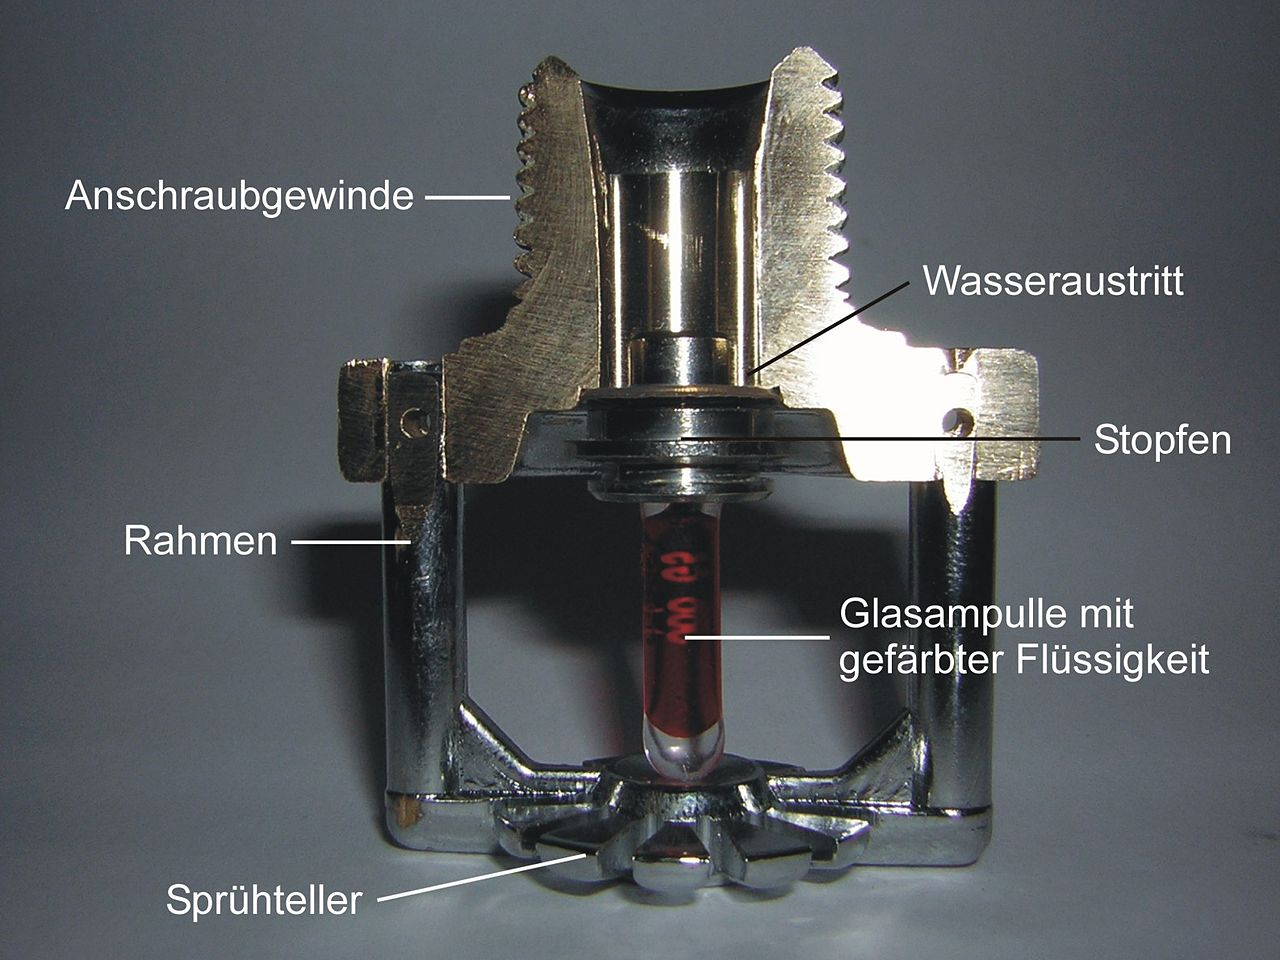
\includegraphics{images/sprinklerkopf.jpg}
    \caption{Aufbau Sprinklerkopf \cite{Sprinklerkopf}}
    \label{fig:AufbauSprinklerkopf}
\end{figure}
Unterschieden wird zwischen Glasfass- und Schmelzlot-Sprinklern. In dieser Arbeit wird auschließlich der gängigere Typ mit Glasfass betrachtet. Außerdem gibt es neben den hier betrachteten hängenden Sprinklerköpfen noch \zB Seitenwand- oder verdeckte Sprinklerköpfe.

Bei der Montage wird der Sprinklerkopf über das Anschraubgewinde mit der Sprinklerleitung verbunden. Nachdem die Sprinkleranlage mit Wasser befüllt wurde, ist der Sprinklerkopf funktionsfähig. Die Glasampulle drückt gegen den Stopfen und verhindert so ein Entweichen des Wassers. Im Brandfall dehnt sich unter Hitzeeinwirkung das Glykolgemisch in der Glasampulle aus und sprengt bei Erreichen der Auslösetemperatur das Gefäß. Der Wasserdruck schleudert den Stopfen aus dem Sitz und das Löschwasser spritzt auf den Sprühteller. Dieser erfüllt die Funktion, das Wasser gleichmäßig in einem bestimmten Radius abhängig von der Raumhöhe und dem Wasservolumenstrom zu verteilen. 


\subsection{Nennöffnungstemperatur}
\label{Ausloesetemperatur}
Die Nennöffnungstemperatur beschreibt die Temperatur des Auslöseelements, bei der die Glasampulle brechen und Wasser aus dem Sprinklerkopf f"|ließen soll. Dabei muss der Hersteller der Auslöselemente nach VdS-Richtlinie 2160:2005 bestimmte Toleranzen beachten (siehe \cite[S. 8]{VDS2160}). Der zulässige Bereich wird bei den verschiedenen Auslösetemperaturen durch ca. $\pm$ 4 \% der Nenn\-öff\-nungs\-temp\-er\-at\-ur eingegrenzt (\zB für 68 °C Nenn\-öff\-nungs\-temp\-er\-at\-ur 65 °C als untere Grenze und 71 °C als obere Grenze). Ob diese Glasfässchen in diesem Toleranzbereich liegen, wird ebenfalls stichprobenartig in einem Flüssigkeitsbad geprüft.
Für verschiedene Anwendungen gibt es entsprechende Auslösetemperaturen. Die Flüssigkeit in dem Glasf"|läschchen wird farblich gekennzeichnet und gibt Aufschluss über die Auslösetemperatur (siehe Tab: \ref{tab:Kennzeichnung}). 
\begin{table}\centering
\caption{Farbliche Kennzeichnung Auslöseelement \cite{VDS4001}}
\label{tab:Kennzeichnung}
\begin{tabular}[width=\textwidth]{@{}ccccccc@{}} \toprule
Orange&Rot&Gelb&Grün&Blau&Malve&Schwarz    \\ \midrule
57 °C&68 °C&79 °C&93-100 °C&121-141 °C&163-182 °C&204-260 °C  \\
\bottomrule
\end{tabular}
\end{table}
Die unterschiedlichen Auslösetemperaturen werden über verschieden große Luftbläschen im Element realisiert. Die Nenn\-öff\-nungs\-temp\-er\-at\-ur sollte mindestens 30 °C über der höchsten Raumtemperatur liegen, sodass es nicht zu einer Fehlauslösung kommt. In ca. 90~\% der Fälle werden im mitteleuropäischen Raum die rot codierten Glasf"|läschchen verwendet. In südlicheren Breitengraden steigt mit höheren Umgebungstemperaturen auch die Bedeutung der gelben Auslöseelemente. Nenn\-öff\-nungs\-temp\-er\-at\-ur\-en von 93~°C bis 100~°C finden oft ihren Platz unter Oberlichtern oder anderen verglasten Flächen. Blaue Glasfässchen werden häufig in industriellen Anwendungen eingesetzt und schwarze Fässchen werden nur in äußersten Ausnahmefällen verwendet.

\subsection{RTI (Response Time Index)}

Der Begriff der Ansprechzeit des Auslöseelements wurde von Heskestad und Bill als "`Response Time Index"' (auch Trägheits-Index genannt) geprägt. Je kleiner der Faktor, desto schneller erwärmt sich das Element und löst im Brandfall aus. Er beschreibt das Produkt aus der thermischen Zeitkonstante $\tau$ für das Auslöseelement und die Wurzel der assoziierten Gasgeschwindigkeit $u$ \cite{Heskestad1989}: 
\begin{equation}
  \text{RTI}=\tau u^{1/2}
  \label{fig:RTI}
\end{equation}
\begin{equation}
    \tau = \frac{mc}{hA} 
    \label{fig:tau}
\end{equation}
Hierbei ist $m$ gleich die Masse, $c$ die spezifische Wärmekapazität, $h$ der Wärmeübergangskoeffizient und $A$ die Oberf"|läche des Auslöseelements. Um den RTI für ein bestimmtes Auslöseelement zu ermitteln, wird die Glasampulle in einem Windkanal einem Luftstrom mit vordefinierten Temperatur- und Geschwindigkeitswerten nach \cite{VDS2160} ausgesetzt. Die bis zum Zerplatzen des Auslöseelements gemessene Zeitspanne wird anschließend zur Berechnung des RTI–Faktors verwendet. Es wird generell zwischen drei verschiedenen Ansprechklassen unterschieden (siehe Tab: \ref{tab:Ansprechklassen}). 

Für Bereiche mit einer hohen Personengefährdung oder Szenarien, bei denen mit einer schnellen Brandausbreitung zu rechnen ist, wird der Einsatz der Klasse "`schnell"' empfohlen \cite{MinimaxInfo}.
Unter realistischen Brandbedingungen verändert sich der RTI im Verlauf des Brandes, obwohl er in den Berechnungen und Simulationen als konstant angesehen wird. Der potentielle Fehler, der hierdurch entsteht, wurde noch nicht hinreichend untersucht \cite[Kap. 4, S. 6]{SFPE3rd}. 
\begin{table}[h]\centering
\caption{Ansprechklassen Auslöseelement \cite{VDS2160}}
\label{tab:Ansprechklassen}
\begin{tabu} to 0.4\textwidth{@{}X[c]X[c]@{}} \toprule
RTI in (m$\cdot$s)$^{0,5}$                    & Ansprechklasse \\ \midrule
< 50        & Schnell        \\
50 - 80     & Spezial        \\
80 - 200    & Standard A     \\
\bottomrule
\end{tabu}
\end{table}

\subsection{C-Faktor}
\label{sec:CFaktor}
Der Wärmeleitungsverlust der Glasampulle an den Sprinklerkopf \bzw an das Sprinklerfitting wird mit dem sogenannten C-Faktor beschrieben. Dieser wurde ebenfalls von Heskestad und Bill im Jahre 1988 \cite{Heskestad1988} eingeführt. Der C-Faktor ist ein Kennwert des gesamten Sprinklerkopfes und nicht der Glasampulle. Er ist in manchen Formeln auch ein Parameter in der Ermittlung des RTI. Da allerdings die Auslöseelemente und Sprinklerköpfe meist von verschiedenen Herstellern produziert werden, wird von den Glasampullenherstellern ein allgemeiner C-Faktor von 0,5 (m/s)$^{0,5}$ angenommen, um eine gewisse Vergleichbarkeit zu garantieren.


Mithilfe der nachfolgenden Formel kann unter konstanten Testbedingungen der C - Faktor in einem Windkanal ermittelt werden:
\begin{equation}
\label{eq:C-Faktor}
    \frac{\Delta T_g}{1+\frac{C}{\sqrt{u_c}}}=\Delta T_{ea}
\end{equation}
dabei ist $\Delta T_{ea}$ die Auslösetemperatur des Glasfässchens, $\Delta T_g$ die Gastemperatur und $u_c$ die Gasgeschwindigkeit. Die Bedeutung des C-Faktors nimmt mit höheren Gasgeschwindigkeiten und -temperaturen \cite{Heskestad1988} ab.





\section{Brandquelle}
\label{sec:Brandquelle}
Die Brandquelle kann aus unterschiedlichen Flüssigkeiten, Feststoffen oder Gasen bestehen. Sie bestimmt wie schnell sich die Brandf"|läche ausbreitet, wie hoch die maximale Wärmefreisetzungsrate ist und wie sich das Rauchgas zusammensetzt.

Bei einem natürlich ablaufenden Brand können verschiedene Brandphasen beobachtet werden. Diese unterscheiden sich in der Wärmefreisetzungsrate $\Dot{Q}$ (siehe Abb. \ref{fig:Brandverlauf}).
Laut VDI 6019 Blatt 1 \cite{VDI6019B1} kann der Brandverlauf in fünf Phasen eingeteilt werden:
\newpage
\begin{setlength}{\leftmargini}{1.85cm}
\begin{description}
    \item[\textbf{Phase 1:}] Brandentstehung mit niedriger Wärmefreisetzungsrate
    \item[\textbf{Phase 2:}] Fortentwickelter Brand mit quadratischer Zunahme der Wärmefreisetzungsrate und Brandf"|läche
    \item[\textbf{Phase 3:}] Stetiger Brand mit konstanter Wärmefreisetzungsrate und Brandf"|läche
    \item[\textbf{Phase 4:}] Kontrollierter Brand bei aktivierter selbsttätiger Löschanlage
    \item[\textbf{Phase 5:}] Brandbekämpfung durch die Feuerwehr
\end{description}
\end{setlength}

\begin{figure}
    \centering
    \includegraphics[width=0.65\textwidth]{images/Brandverlauf.pdf}
    \caption{Möglicher Brandverlauf bei Sprinklerauslösung \cite{VDI6019B1}}
    \label{fig:Brandverlauf}
\end{figure}

Für die Berechnung der Sprinklerauslösezeiten in der VDI-Richtlinie wird ausschließlich die zweite Phase für hochenergetische Brände betrachtet. Die erste Phase f"|ließt aufgrund der niedrigen Wärmefreisetzungsrate nicht in die Berechnung ein und die dritte Phase wird nicht beachtet, da davon ausgegangen wird, dass der Brandherd nicht seine maximale Wärmefreisetzungsrate erreicht und davor die Sprinkleranlage auslöst. 
\begin{table}[b!]\centering
\caption{Brandintensitätskoeffizienten \cite{VDI6019B1}}
\label{tab:Brandintensitätskoeffizient}
\begin{tabu} to 0.68\textwidth{@{}X[1,c]X[1.4,c]@{}} \toprule
Geschwindigkeit der Brandentwicklung    & Brandintensitätskoeffizient $\alpha$ ($kW/s^2$)\\ \midrule
Langsam     & 0,0029        \\
Mittel      & 0,012        \\
Schnell     & 0,047       \\
Sehr schnell& 0,188       \\
\bottomrule
\end{tabu}
\end{table}
In Phase 2 läuft die Wärmefreigabe quadratisch ab und der sogenannte Brandintensitätskoeffizient $\alpha$ wird benutzt, um den Brandverlauf abzubilden. Die Formel für die Wärmefreisetzungsrate $\Dot{Q}$ zum Zeitpunkt $t$ in Phase 2 lautet: $\Dot{Q}(t)=\alpha \cdot t^2$. 
Dies gilt als eine realistische Methode, um verschiedene Brandherde zu beschreiben \cite{SFPE5th}. Hierbei wird zwischen verschiedenen Geschwindigkeiten der Brandentwicklung unterschieden (siehe Tab: \ref{tab:Brandintensitätskoeffizient}).



\section{Geometrie des Raumes}
\label{Geometrie}
Ein weiterer erheblicher Einf"|lussfaktor für die Auslösezeit eines Sprinklerkopfes ist die Geometrie des Raumes. Während ein Unterzug an der Decke das Voranschreiten des Rauchgases zeitlich verzögern oder umleiten könnte, hätte eine zum Sprinklerkopf geneigte Deckenschräge den gegenteiligen Effekt. Hierbei würde der Rauch sich nicht radial an der Decke ausbreiten, sondern abhängig vom Deckenwinkel, den Rauch prädesteniert in eine Richtung des Raumes lenken. So könnte es zu einer schnelleren Auslösezeit kommen. Montagevorgaben und Einbauhinweise für all diese unterschiedlichen räumlichen Gegebenheiten werden in der VdS~CEA~4001 betrachtet. 

Die Rasterabstände $S$ zwischen den Sprinklern variieren je nach Brandgefahrenklasse, betragen jedoch maximal 4,6 Meter \cite[S. 100]{VDS4001}. In Abb. \ref{fig:Sprinkleranordnung} sind zwei unterschiedliche Anordnungen von Sprinklerköpfen zu erkennen. 
Um den horizontalen Abstand $r$ zwischen Brandherd und Sprinklerkopf zu ermitteln, muss vom ungünstigsten Fall ausgegangen werden. Dieser tritt ein, wenn der Brandherd genau in der Mitte zwischen vier Sprinklerköpfen liegt (siehe Abb. \ref{fig:Sprinklerabstand_genau}). Nach dem Satz des Pythagoras kann mithilfe folgender Formel der Abstand $r$ ermittelt werden: 
\begin{equation}
    r=\sqrt{\left ( \frac{S}{2} \right )^2+ \left ( \frac{S}{2} \right )^2}
\end{equation}
und durch Einsetzen des maximalen Rasterabstandes $S$:
\begin{equation}
    r=\sqrt{\left ( \frac{4{,}6 m}{2} \right )^2+ \left ( \frac{4{,}6 m}{2} \right )^2}= 3{,}25 m
\end{equation}

Bei Lagerhallen oder Sälen kann der senkrechte Abstand mehrere Meter betragen. Je höher dieser ist, desto mehr Umgebungsluft wird durch Induktion in den Plume über dem Brandherd gemischt und kühlt den Rauch ab. 
\begin{figure}
    \centering
    \includegraphics[trim=0 2cm 1cm 0,clip,width=\textwidth]{images/Sprinklerabstand.pdf}
    \caption{Abstände zwischen Deckensprinklern mit $S$ und $D$ nach \cite{DIN12845}}
    \label{fig:Sprinkleranordnung}
\end{figure}
\begin{figure}
    \centering
    \includegraphics[width=0.7\textwidth]{images/Sprinklerabstan_genau.pdf}
    \caption{Maximaler Abstand $r$ zwischen der Mitte des Brandherdes und des Sprinklerkopfes.}
    \label{fig:Sprinklerabstand_genau}
\end{figure}
Die Raumtemperatur und somit die Sprinklerkopftemperatur zum Zeitpunkt $t=0$ muss ebenfalls berücksichtigt werden. Je größer die Differenz zwischen der Umgebungs- und Auslösetemperatur, desto länger dauert die Sprinklerauslösung. Für konservative Simulationsergebnisse sollte generell die niedrigste mögliche Umgebungstemperatur für die Berechnung \bzw Simulation verwendet werden \cite{SFPE5th}. Wenn \zB am Wochenende die Raumlufttemperatur von $20$ auf $15\,^{\circ}\text{C}$ abgesenkt wird, sollte letztere als die Anfangs\-temperatur angenommen werden. 



